
%\documentclass[10pt, conference, compsocconf, draft]{IEEEtran}

\documentclass[10pt, conference, compsocconf]{IEEEtran}


\IEEEoverridecommandlockouts

\usepackage{balance}
\usepackage{graphicx}
\usepackage{url}
\usepackage{xcolor}
\usepackage{multirow}
\usepackage{epsfig}

\usepackage[dvips]{hyperref}
\usepackage{cite}

\hypersetup{
  bookmarks = false,
  pagebackref=true,
  pdftoolbar=true,
  pdfnewwindow=true,
  pdfmenubar=true,
  pdftitle = {Source Camera Identification in Real Practice: a Preliminary Experimentation},
  pdfkeywords = {Image Forensics; PRNU; Digital Forensics; Digital Camera Identification; Digital Camera Model Identification; Digital Investigations},
  pdfauthor = {Aniello Castiglione, Giuseppe Cattaneo, Maurizio Cembalo, Umberto Ferraro Petrillo},
  pdfsubject =  {The First International Workshop on Cloud, Wireless and e-Commerce Security - CWECS 2010},
  pdfcreator =  {Dr. Aniello Castiglione - castiglione@ieee.org},
}



\newcommand{\Lukas}{Luk{\' a\v s} {\em et  al.}}

% correct bad hyphenation here
\hyphenation{op-tical net-works semi-conduc-tor}


\begin{document}
%
% paper title
% can use linebreaks \\ within to get better formatting as desired
\title{Source Camera Identification in Real Practice: a Preliminary Experimentation
\thanks{The project is a joint work with the CNCPO (\textsl{Centro Nazionale per il Contrasto 
della Pedopornografia Online}), part of the ``Dipartimento della Pubblica Sicurezza'' within 
the Italian Ministry of Interior.}
}

%Realizzazione ed analisi sperimentale di uno strumento per la source camera identification

% author names and affiliations
% use a multiple column layout for up to two different
% affiliations

\author{
\IEEEauthorblockN{Aniello Castiglione\thanks{Corresponding author: Aniello Castiglione,~Member,~\textit{IEEE},~\href{mailto:castiglione@ieee.org}{castiglione@ieee.org},~Phone: +39089969594,~FAX: +39089969821}, Giuseppe Cattaneo and Maurizio Cembalo}

\IEEEauthorblockA{Dip. di Informatica ed Applicazioni ``\textit{R.M. Capocelli}''\\
Universit\`{a} di Salerno\\
Via Ponte don Melillo, I-84084 Fisciano (SA), Italy\\
Email: \href{mailto:castiglione@ieee.org}{castiglione@ieee.org} \{cattaneo, maucem\}@dia.unisa.it}

\and
\IEEEauthorblockN{Umberto Ferraro Petrillo}
\IEEEauthorblockA{Dip. di Statistica, Probabilit\`a e Statistiche Applicate\\
Universit\`a di Roma ``Sapienza''\\
P.le Aldo Moro 5, I-00185 Rome, Italy\\
Email: \href{mailto:umberto.ferraro@uniroma1.it}{umberto.ferraro@uniroma1.it}}
}

%%\author{\IEEEauthorblockN{Authors Name/s per 1st Affiliation (Author)}
%%\IEEEauthorblockA{line 1 (of Affiliation): dept. name of organization\\
%%line 2: name of organization, acronyms acceptable\\
%%line 3: City, Country\\
%%line 4: Email: name@xyz.com}
%%\and
%%\IEEEauthorblockN{Authors Name/s per 2nd Affiliation (Author)}
%%\IEEEauthorblockA{line 1 (of Affiliation): dept. name of organization\\
%%line 2: name of organization, acronyms acceptable\\
%%line 3: City, Country\\
%%line 4: Email: name@xyz.com}
%%}
% make the title area
\maketitle


\begin{abstract}
%Nowadays, the spread and the pervasiveness of digital photography have reached
%levels that were unthinkable until some years ago. This phenomenon has been fostered by
%many online services (e.g., PicasaWeb, Facebook) that offer to the general public the 
%possibility to share and exchange their photos in a convenient and easy way. As a side effect, it is 
%common to find in Law prosecutions a digital evidence that consists in a digital photo. This
%led to the origination of a new discipline, the Image Forensics, that helps investigators in dealing with digital images.
%A typical problem that is studied by this discipline is the source camera identification problem,
%i.e., identifying the camera that has been used to generate a digital picture.
%To this end, many identification techniques have been proposed and experimented so far. 
%However, most of these experimentation have been conducted under the unrealistic assumption
%that the images to be processed were not previously processed or modified. 

In this paper, we present an experimental evaluation of one of the most effective source camera identification technique proposed so far, the technique by Luk{\' a\v s} {\em 
et  al.}. This method uses the characteristic noise left by the sensor on a digital picture as a fingerprint in order to identify the source camera used to take that picture. 
The goal of our experimentation is to assess the effectiveness of this technique when used with pictures that were previously modified using several common image-processing functions coming with photo-editing tools.  Our results seem to confirm that, in most cases, the method by \Lukas\ is resilient to the modifications introduced by the considered image-processing functions. However, we were able to pinpoint some cases where the quality of the identification process deteriorated because of the noise introduced by the pre-processing.

%Since this technique has been conceived as a tool to
%support investigations, the result is acceptable only if it comes with the highest 
%degree of accuracy. 
%
%We first implement a framework to perform an experimental analysis of such a technique 
%and to test its practical viability against our specific purposes assuring the necessary reliability.
%Second, we analyze the behaviour of the Luk{\' a\v s} method when in presence of image
%editing operations. We notice that the Luk{\' a\v s} proposal could be improved to obtain better results.
%This work intend to be the first contribution in the Image Forensics panorama
%which implements in the real world the theoretical assumption of this emerging science.   


%
%We first implemented a framework to perform an experimental 
%analysis of such a technique and to verify on the field if it could be successfully used 
%for our specific purposes with the necessary reliability.
%

% Our main goal is to develop a a full fledged system prototype (a tool set supported 
% by a robust methodology) able to give a solution for the problem of the identification 
% of the camera, among a predefined set, that shot a given image.

% The project started from the results presented by Lukas  {\em et  al.}  which use the characteristic noise 
% of the sensor as a fingerprint to identify 
% the source camera. We first implemented a framework to perform an experimental 
% analysis of such a technique and to verify on the field if it could be successfully used 
% for our specific purposes with the necessary reliability. Afterwards we implement a graphical 
% application easy to be used by investigators.

% In this paper we present also the system components of the application and the results of our experimentation.

\end{abstract}


\begin{IEEEkeywords}
Image Forensics; PRNU; Digital Forensics; Digital Camera Identification; Digital Camera Model Identification; Digital Investigations.
\end{IEEEkeywords}


\section{Introduction}
% This section will introduce the general problem of digital camera
% identification and its applications to the field of digital forensic. 
% Moreover, we will discuss about existing contributions in the
% following terms.

% Several approaches have been proposed so far to this end. Many of
% these approaches have also been experimented using large sets of
% digital images. 

In the digital era, the creation and the modification of images (as well as videos) can be performed at a very low cost with simple editing tools which are widely and easily accessible to everyone. As a consequence, it is not possible to always consider authentic an image or a video. This simple fact may become an issue if an image or a video is a digital evidence involved in a Law investigation. 

The Image Forensics discipline tries to help the investigators when in presence of digital photographic evidence. One of the many questions that the Image Forensics tries to respond is the {\em source camera identification problem}, i.e., establish if a given image has been taken from a given digital camera. Many identification techniques have been proposed so far in literature. All these techniques generally work by using the sensor noise left by a digital sensor when taking a picture as a fingerprint for identifying that sensor. These works are generally accompanied with experiments proving the effectiveness of these techniques, both in terms of False Acceptance Rate (FAR) and False Rejection Rate (FRR).  Unfortunately, most of these contributions do not take into consideration  that, in the real practice, the images that are shared and exchanged through the Internet have often been pre-processed. Instead, it is a common practice to assume, in these experimentations, that the images to be examined are unmodified or, at most, to ignore the effects of the pre-processing.


% Ho sfumato un po' sul discorso Flicker perch�, a differenza di Facebook, c'� pi� attenzione verso la % quale della foto e comunque l'utente ha la possibilit� di memorizzare il raw (se ricordo bene)
% Al contrario, FB procede con un resize incondizionato della foto, su cui l'utente non ha controllo
Even without considering the case of malicious users that could intentionally process a picture in order to fool the existing identification techniques, this assumption is unrealistic for at least two reasons. The first is that, as we were saying before, almost all existing photo-managing software offer several functions for adjusting,  sometimes in a ``magic'' way (see the ``I'm feeling lucky'' function
on Google Picasa~\cite{picasa}),  several characteristics of a picture. The second reason is in the way the images are managed by some of the most important social networks and image publishing sites. These services usually make some modifications to the original photos before publishing them
in order to improve their appearance or to reduce their size.
The contribution of this paper represents a preliminary work to try to figure out how
one of the most prominent source camera identification technique responds when in presence of pre-processed images. 
%For example,  in the 2009, only on Facebook have been uploaded 2.5 billion photos each month r~\cite{facebook}.

%How the existing Image Forensics techniques do manage, if they do it, such 
%elaborations? How such elaborations alter the identification of a digital photos?

\subsection{Organization of the Paper} 
In Section \ref{sec:did} we will provide some basic definitions about the source camera identification problem and we will briefly review the existing literature on this topic. In Section \ref{sec:luk} we will introduce in the details the identification technique presented by Luk{\' a\v s} {\em et  al.}  in \cite{Lukas06} and based on the Photo-Response Non-Uniformity
(PRNU) of both CCD~\cite{Janesick95} and CMOS sensors~\cite{Holst96}.
In Section \ref{sec:exp} we present the results of an experimentation of this technique performed on a test-bed of nearly 1500 images taken from 8 different cameras. In our experiments, we compared the performance of this technique when applied to the identification of the cameras used to take both modified and unmodified pictures. Finally, in Section \ref{sec:conc} we sketch some concluding remarks. 
%The source code for our software implementation and the images used in our experimentation
%are available for download at the following address ... (???)

\section{Digital Camera Identification}
\label{sec:did}
% First, we introduce and define the problem of digital camera
% identification.

% Second, we review the several different approach/variables that can be used to
% identify the camera and/or the camera model used to take a photo. 

% Third, we discuss the scientific works implementing the approaches
% introduced above, with a particular emphasis on papers with an
% experimental part.

Each digital picture contains a random component of
noise and a deterministic component, the {\em pattern noise}, that
depends on the sensor used to shoot the picture. The pattern noise is
very similar within all the pictures taken by the same sensor. 


The problem of digital camera identification concerns with the
identification of the camera that has been used to generate a digital picture, by examining the pattern noise existing in that picture.  Such a technique is called {\em source camera identification} and has not be confused with the more general {\em digital camera model identification} problem,  in which we are just interested in  establishing which camera model has been used to take a certain picture. 


Up to now, three are the main approaches proposed in literature 
for the source camera identification problem. These approaches differ in the
type of pattern noise that is used. 

% Inhomogeneity mi suona un po' male, Maurizio, sei sicuro che se ne parli in questi termini nei vari 
% articoli?

The first approach uses the {\em Photo-Response Non-Uniformity} (PRNU)
noise, i.e., the noise produced by the sensor due to the inhomogeneity of 
the silicon wafers used to build it. Luk{\' a\v s} {\em et  al.}~\cite{Lukas06} and Chen {\em et al.}~\cite{Chen08}
proposed two methods for identifying source camera based on the
PRNU.  These techniques can be used to isolate and extract this noise from a set of pictures taken with a same camera, and use this noise to match or not the cameras with the photos under investigation. Their results show that these methods have high detection rates.
Goljan {\em et al} in \cite{Goljian09} used a refinement of  the method of Chen
to run a digital camera identification experiment on a massive
database of digital pictures downloaded from the Internet.   

The second approach uses the lens radial distortion that causes
straight lines to appear as curved lines on the output images. Choi {\em et al.} have tried this method
 in~\cite{Choi06}. As a result, they discovered that this method failed to measure
the radial distortion except when there are explicit straight lines in the picture to be processed.

The last approach relies on the CFA (\emph{Color Filter Array}) interpolation, which is a technique
used by digital cameras after a picture has been taken in order to
determine the colors of the scene. This technique produces small
non-uniform color zones that can be seen as a noise
source. Each camera has its interpolation algorithms and each
algorithm produces a small degree of noise that, generally, slightly
changes from camera to camera.
Bayram~{\em et al.} in~\cite{Bayram05} explored the CFA interpolation process to
determine the correlation structure present in each color band which
can be used for image classification. 
In this direction, Kharrazi~{\em et al.} in~\cite{Kharrazi04} and Long and 
Huang in~\cite{Long06} proposed two methods. The first method identifies a set of
image features that can be used to uniquely classify a camera model. 
The accuracy of this method decreases as the number of cameras increases. 
The second method obtains a coefficient matrix from a quadratic pixel correlation model
 where spatially periodic inter-pixel correlation follows a quadratic form. 
The experimental result seems to suggest that these two methods work better for the camera model 
identification problem rather than for the source camera identification problem.

% The sensor of a digital camera can only capture the luminance of a scene, not its colors. This
% information is determined by the CFA interpolation technique applied
% on the picture after this has been taken. 


% the noise produced by the {\em imperfections}
% \cite{Janesick95, Holst96} existing in every digital camera sensor as
% a fingerprint for tracing back to the camera used to shoot a picture.

% In the image acquisition process there are numerous sources of
% imperfections and noise. 

% The pattern noise is made up two main
% components: the {\em fixed pattern noise} (FPN) and the {\em
%   photo-response non uniformity noise} (PRNU).  The FPN is the
% variation of the pixel response of an image sensor in the dark; under
% these conditions particular pixels of the sensor, depending on
% exposure and temperature, are susceptible to giving brighter
% intensities. The PRNU 
% properties on the sensor.

%   The
% effect of these distortions on the resulting picture may be considered
% as the fingerprint for a digital camera.


\section{The Approach by Luk{\' a\v s} {\em et  al.}}
\label{sec:luk}

% Una delle migliori tecniche in letteratura
We focus our attention on the approach proposed by Luk{\' a\v s} {\em et  al.}
because is one of the most effective method, and is not as expensive
in terms of hardware resources as other similar methods such as the one proposed by Goljan in~\cite{Goljian09}.

% Come funziona la tecnica
The approach by Luk{\' a\v s} {\em et  al.} works in two stages. In the first
stage, the PRNU associated with a CCD sensor is determined by
analyzing a batch of images taken with that sensor. In the second
stage, given a picture, the procedure evaluates the correlation between 
the noise existing in that picture and the pattern noise evaluated in the previous stage
in order to discern if such a picture has been taken using that CCD sensor.


The extraction of the PRNU from an image is performed by denoising the
image using  a wavelet-based algorithm. 
The denoised image is subtracted by the original image giving as output a new
image containing several components: the CCD sensor noise, the random noise 
and various contributions from image signal.
Hence, to eliminate the random component of the noise,
the denoising procedure is applied to a set of images (captured by the
same camera) and the corresponding noise residues are averaged to
obtain the reference pattern of a given digital camera. 

Afterwards, to determine whether a given image is captured by a digital camera,
the noise pattern extracted from the given image is correlated with
the reference pattern of the camera.  If the correlation value exceeds
a pre-determined threshold, then the image was taken with that camera. To
estimate the accuracy of the method and to compute the thresholds,
they used the Neyman-Pearson criterion, specifying a bound on the FAR.

%I loro risultati

%This method has proven to be robust, and has also been witnessed by
%the experimentation conducted by Luk{\' a\v s} {\em et  al.}.
%However, Luk{\' a\v s} {\em et  al.} did not take in account an important issue. 
%Nowadays, it is unlikely that pictures taken using a digital camera are published
%or exchanged without first applying any sort of modification or
%resizing. Indeed, the possibility of retouching photos are 
%endless due to image editing applications currently
%available. Such applications have plenty of options for improving the quality 
%of a picture or simply for reducing its size. 
%
%The question that arises is: is the technique
%proposed by Luk{\' a\v s} {\em et  al.} resilient to these modifications? 
%In the remaining part of this paper we will try to answer to this
%question by testing this classification technique over a test set of
%pictures that have been previously processed using several common
%functions such as {\em auto level adjustment} (i.e., automatically correct 
%the tonal values in a photo), {\em auto contrast} (i.e., automatically improve 
%the contrast of a photo), {\em auto color adjustment} (i.e., automatically examine 
%a picture and remaps the colors of a picture), and {\em resizing} (using three
%different types of resizing).
%

\subsection{Our Implementation}

We implemented the method proposed by Luk{\' a\v s} {\em et  al.} using the 
Matlab software \cite{MatlabSITE}. We decided to use this software because of its efficiency
and because it provides several pre-implemented components (e.g. wavelets functions) which are useful in the implementation of the various identification techniques. 

Concerning the implementation, the main ingredient of the method proposed by Luk{\' a\v s} {\em et  al.} is the PNRU filter.  This filter simulates the behavior of the Wiener filter in the wavelet domain and it has been  suggested in~\cite{Mihcak99}. The Wiener filter is based on a statistical approach and aims to filter the noise of an image.

There exist several families of wavelets, each one suitable for different application and differing 
in the number of coefficients they use. In early stages of our experiments, we tried several combinations and find out that the optimal choice was represented by 4-levels and 8-levels Daubechies wavelets.
% Fridrich usa 8-tab Binomial-QMF (Also referred to as Daubechies wavelet)


\section{Experimental Analysis}
\label{sec:exp}

We organized our experiments in three phases. In the first phase, we were interested in assessing the effectiveness of the method by Luk{\' a\v s} {\em et  al.} when applied to the camera identification for unmodified digital pictures. In the second phase, we first pre-processed the original set of pictures using several types of image-processing functions and then repeated the identification process using the decision thresholds determined during the first experiment according to non pre-processed images. In the third phase, we repeated the previous experiments with pre-processed images using, this time, decision thresholds that have been generated starting from pre-processed images.
In all experiments we considered seven different camera models, resulting in eight cameras (as shown in Table~\ref{cameras}). In order to stress the identification method and to cover a wider range of hardware, we choose cameras belonging to different
market sectors and different manufactures. Looking at Table~\ref{cameras}, cameras with ID 1 and 2 have been chosen because  they have the same image sensor size and because we believe that they have the same CMOS sensor~\cite{EOS1000}. Cameras with ID 3 and 4 share the same brand and model. The other four cameras are a mix of common cameras. 

% Lascerei fuori la frase che segue dal momento che nella nostra successiva analisi non abbiamo mai tenuto conto di questo aspetto. 
%All eight cameras have different production year, in order to verify if newer
%cameras carry with them a reasonable level of noise which is enough for applying our methods.\\

%%In all our experiments we considered seven different camera models, reported in the table \ref{cameras}. In order to stress the identification method, we have been using two couple of cameras of different models but with the same manufacturer, plus two cameras of the same model and two cameras having two different manufacturers.

\begin{center}

\begin{table}[hbt]
\centering
\caption{Cameras used in our experimentations}
\begin{tabular}{ | l | p{2.2cm} | l | l |} 

\hline
\textbf{ID} & \textbf{Model} & \textbf{Sensor type} & \textbf{Image size}  \\ \hline \hline
1 & Canon EOS 400D 				& CMOS 	& 3888x2592 \\ \hline
2 & Canon EOS 1000D 				& CMOS  	& 3888x2592 \\ \hline
3 & Canon PowerShot A400 instance A 	& CCD  	& 2048x1536  \\ \hline
4 & Canon PowerShot A400 instance B 	& CCD 	& 2048x1536  \\ \hline
5 & Panasonic Lumix DMC-FZ20 		& CCD 	& 2048x1536  \\ \hline
6 & Panasonic Lumix DMC-FS5 		& CCD 	& 3648x2736  \\ \hline
7 & Kodak EasyShare CX 7530 		& CCD 	& 2560x1920  \\ \hline
8 & HP PhotoSmart E327 				& CCD 	& 2560x1920  \\ \hline
\end{tabular}\label{cameras}
\end{table}

\end{center}

For each camera model $c \in C=\{1, 2, \dots, 8\}$ we collected two set of images: the {\em Images for Reference Pattern} (IRP) and the {\em Images for Testing} (IT). We denote with IRP$_{c}$ / IT$_{c}$ the IRP / IT sets for the camera $c$. The IRP$_{c}$ set is composed of 128 images collected by taking pictures of a uniform white surface. The images have been taken on a tripod, with no flash, auto-focus, no-zoom, best JPEG compression quality, and with all the other options set to their default values. The IT$_{c}$ set is made of 64 images portraying different types of subjects. In this case, the images have been taken using different types of settings, with the exception of the JPEG compression quality and of the image size, both always set to maximum. 


% Le formule che seguivano non mi pare aggiungessero qualcosa a quanto gi� detto. Nemmeno facciamo pi� uso di questa notazione nel resto del paper, e quindi possiamo evitare di definire tutte queste cose e sfruttare lo spazio che si libera per ingrandire una delle due figure.
%
%\[C=\{ID01, ID02, \dots, ID02\}\]
%\[\forall c \in C, ~~~~~~~ \left | IT_{c} \right | = 64, ~~~~~~~ \left | IRP_{c} \right | = 64\]\\
%
%The dataset of the image for testing IT is $D_{IT}$ which can be formalized as: \[D_{IT} = \bigcup_{c \in C} IT_{c}\] resulting in:
%
%\[\left | D_{IT} \right | = \sum_{c \in C} \left | IT_{c} \right |  = \left | C \right | * \left | IT_{c} \right | = 8 * 64 = 512\]
%
%while the dataset of the image reference pattern (IRP) is $D_{IRP}$ and can be formalized as: \[D_{IRP} = \bigcup_{c \in C} IRP_{c}\] resulting in:
%
%\[\left | D_{IRP} \right | = \sum_{c \in C} \left | IRP_{c} \right |  = \left | C \right | * \left | IRP_{c} \right | = 8 * 128 = 1024\]

%%%\[ IRP_{total}=\sum_{c \in C} \left | IRP_{c} \right |   ~~~C \in \{ID01, ID02, \dots, ID08\} \]
%%%
%%%resulting in \[ \left | IRP_{c} \right | * \left | C \right | = 128 * 8 = 1024 \]
%%%
%%%\[ IT_{total}=\sum_{c \in C} \left | IT_{c} \right |   ~~~~~~~C \in \{ID01, ID02, \dots, ID08\}  \]
%%%
%%%resulting in \[ \left | IT_{c} \right | * \left | C \right | = 64 * 8 = 512 \]


The effectiveness of the identification has been measured by counting the number of pictures erroneously rejected by the identification technique over the total number of pictures taken with a certain camera (FRR). Moreover, in all our experiments we have set our decision thresholds in such a way to keep to $0$ the total number of pictures erroneously classified as taken with a certain camera (FAR). All the experiments have been run on a server equipped with two 4-core Intel Xeon X7350 processors at 2.93GHz and using the Linux Ubuntu O.S.


%In order to see the effectiveness of the implemented method, we conducted several experiments.
%After we found that the method works well, we have tested it on various operators to check the goodness.
%We chose the dataset of images and all tests were performed on this set. In the presentation of results,
% in addition to the value of FRR was also indicated the number of images not recognized. 
% This indicator allows us an immediate reading and comparing data.
%In this section we describe first the cameras used and the way we followed to create the image sets. 
%Secondly what kind of experiments we performed in.






\subsection{Experiment 1}\label{exp1}


% We present and discuss the results of the experiments conducted on the image
% set using our implementation of the tecnique proposed by Lukas {\em
%   et al}, using the following experiments:
% \begin{itemize}
% \item{}images matching the camera fingerprint.
% \item{}Error rates computed from the FAR and FRR.
% \end{itemize}

A preliminary problem to be faced when applying the method by Luk{\' a\v s} {\em et  al.} is to ensure that the two images to be correlated (i.e., the image reference pattern and the image to be identified) must have the same size. This condition can be easily met in three different ways:

\begin{itemize}
\item{\bf Sub}: extract from both images two subimages of the same size
(e.g., extract two images originating at point $(0,0)$ and having size 512x512);
\item{\bf Crop}: crop the larger image to match the smaller image;
\item{\bf Resize}: resize the larger image to match the smaller image;
\end{itemize}


\begin{table*}[bht]
\centering
\caption{Decision thresholds, FRR and number of images rejected on the red channel for the experiments Sub, Crop and Resize.}
\begin{tabular}{  | p{1.8cm}   | p{1.8cm} | p{1.8cm}  |  p{1.8cm} | p{1.8cm}  | p{1.8cm} | p{1.8cm}  |} 
\hline
& \multicolumn{2}{|c|}{ \textbf{Sub} } & \multicolumn{2}{|c|}{ \textbf{Crop} }  & \multicolumn{2}{|c|}{ \textbf{Resize} }\\ \hline
{\textbf{ID}}& Decision threshold& Images rejected (FRR) & Decision threshold& Images rejected (FRR) & Decision threshold& Images rejected (FRR)  \\ \hline

1 &	0,0120 	& 	|			& 0,0095	& |			&	0,0095	&	| \\
2 &	0,0120 	& 	2 (0,0313)		& 0,0122	& |			&	0,0122	&	| \\ 
3 &	0,0216  	& 	5 (0,0781) 	& 0,0188	& 3 (0,0469)	&	0,0188	&	3 (0,0469) \\ 
4 &	0,0243  	& 	2 (0,0313) 	& 0,0333	& |			&	0,0333 	&	| \\ 
5 &   0,0705  	&	|			& 0,0826	& |			& 	0,0826 	&	| \\
6 &	0,0222  	&	2 (0,0313)		& 0,0187	& |			&	0,0187 	&	| \\ 
7 &	0,0124  	&	62 (0,9688)	& 0,0026	& 38 (0,5938)	&	0,0061	&	| \\
8 &	0,0420  	&	|			& 0,0226	& |			&	0,0226 	&	| \\ \hline \hline
\multicolumn{2}{|c|}{total number of images rejected} & 73& & 41 & & 3 \\
\hline
\end{tabular}
\label{db8SubCropResize}
\end{table*}



 \begin{figure*}[hbt]
 \centerline
 {
 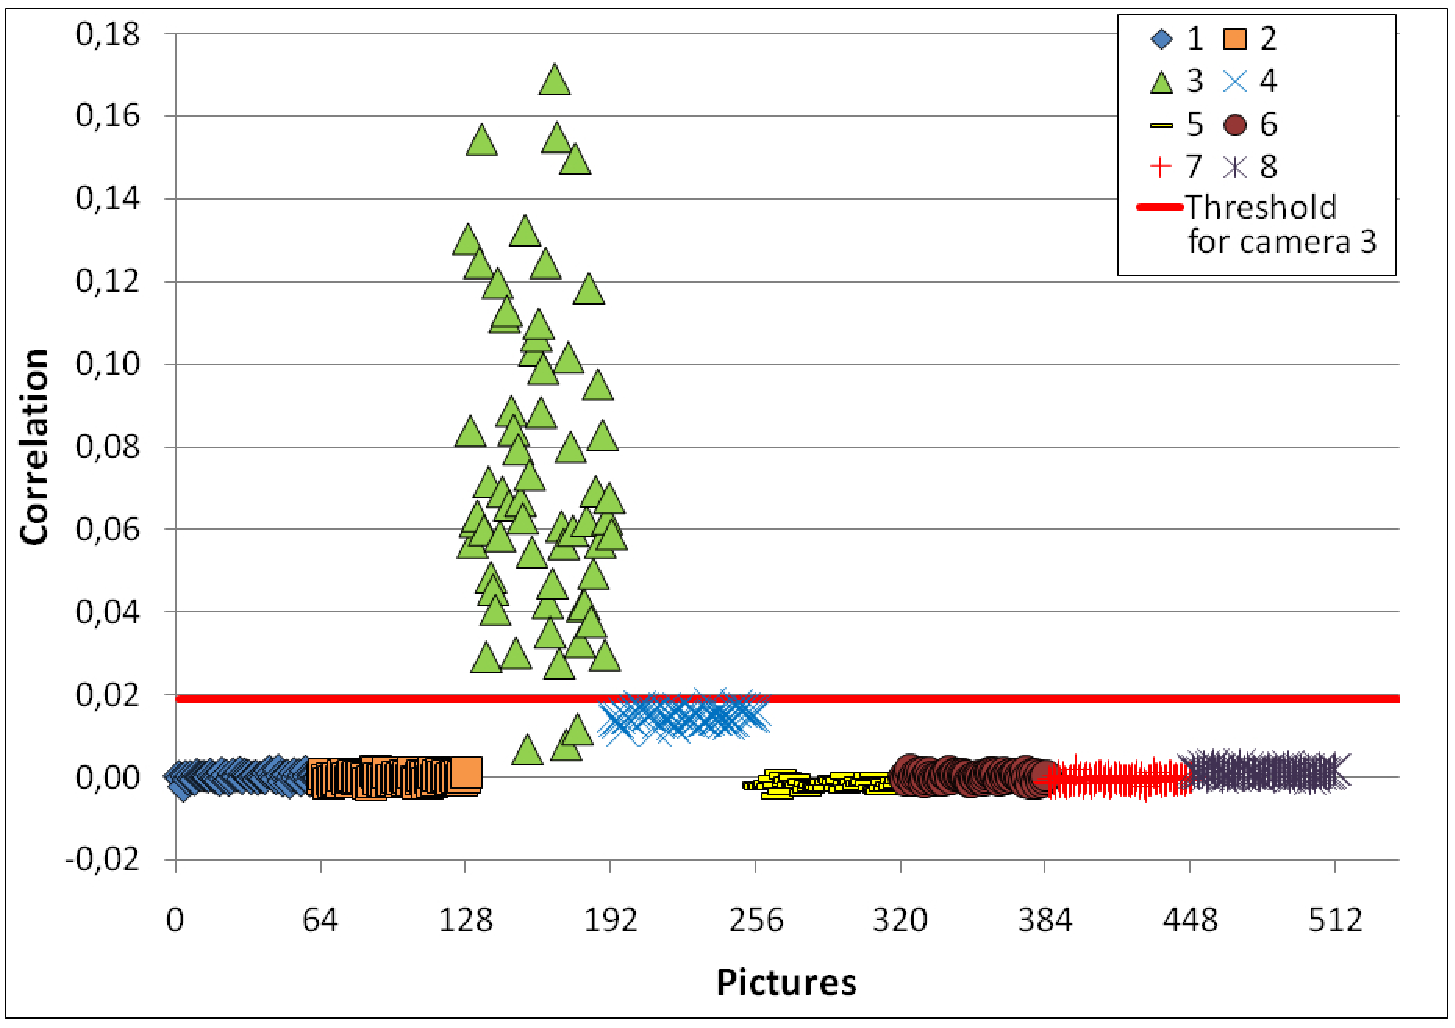
\includegraphics[width=12.0truecm]{A400_64Color.pdf}}
 %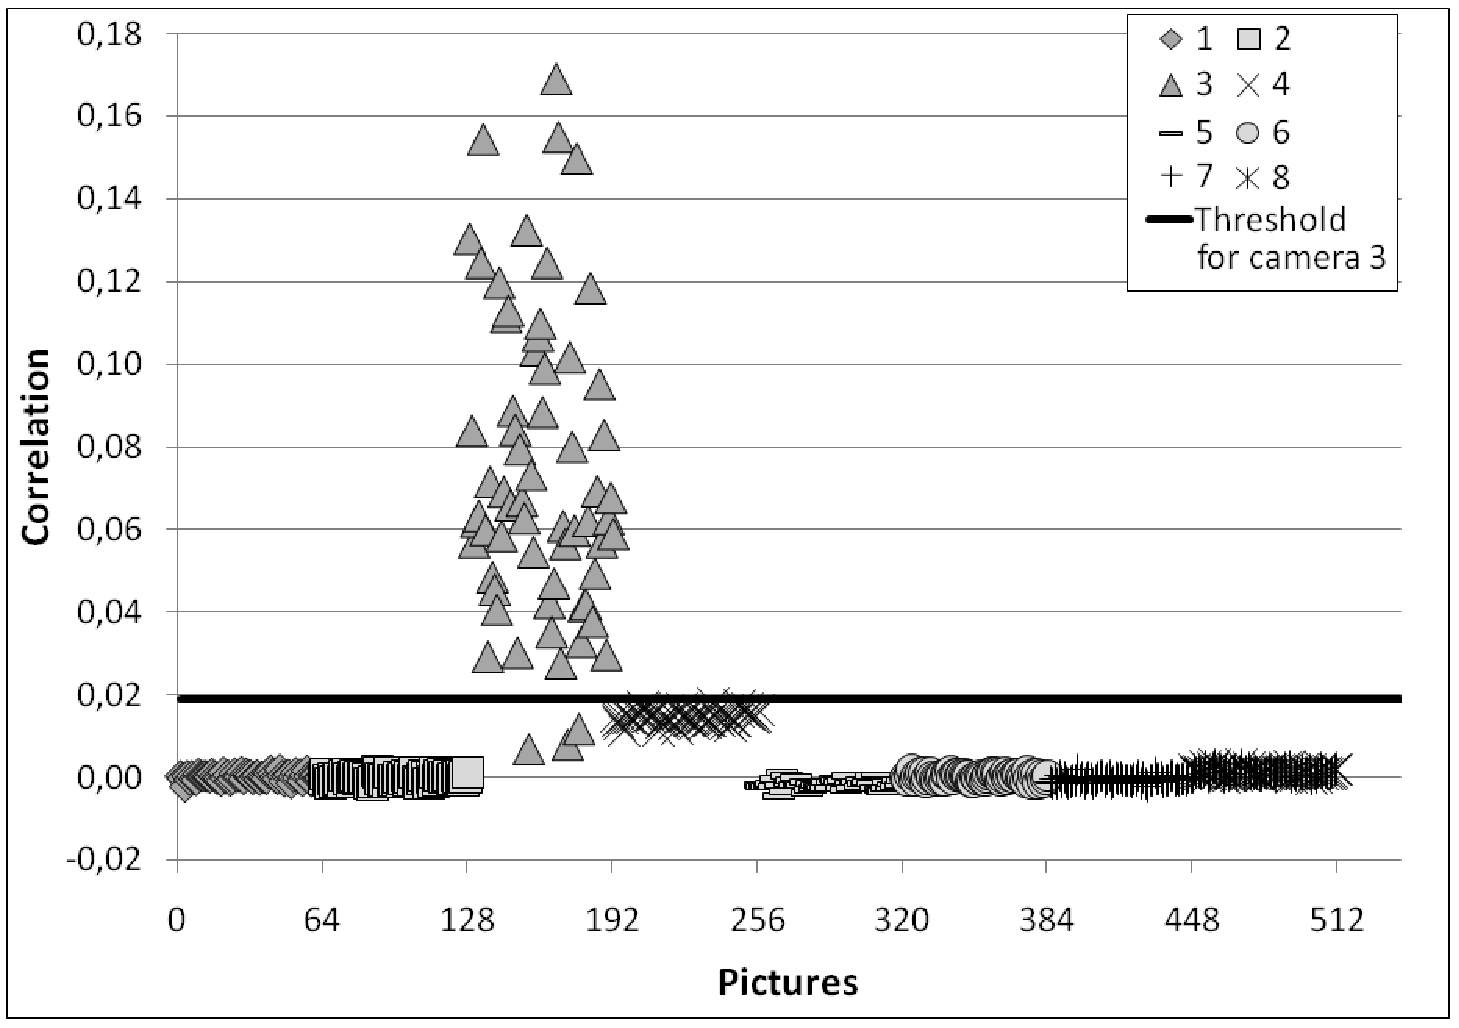
\includegraphics[width=12truecm]{A400_64Gray.pdf}}
 \caption{Scatter plot of the correlations between all the images of the data set and the Image Reference Pattern of the camera with ID 3.}
 \label{scatterPlot}
 \end{figure*}


The original method proposed by Luk{\' a\v s} {\em et  al.} uses the {\bf Crop} approach. In our case, we decided to test also the other two approaches in order
to determine which one performs better. According to our experiments, presented in Table~\ref{db8SubCropResize},  the best approach seems to be {\bf Resize} while the worst is {\bf Sub}. The reason for such a bad performance is likely to reside in the elimination of a large part of the original image, performed by this technique when processing large pictures. The average resolution of the pictures used in our experiments is near 2560x1920. As a consequence of this, the cropped image, whose size is fixed to 512x512, retains only the 5\% of the original image and of its signature, and thus is subject to a worst correlation. In all the remaining experiments presented in this paper, we will always use, when needed, the {\bf Resize} technique.


%
%For each of the points above we performed an experiment, naming 
%respectively {\em EX1-512x512}, {\em EX2-Crop} and {\em EX3-Resize}, to see which 
%of the three approaches was the best.
%
%In the method presented by Lukas {\em et al.}, to calculate the correlation, 
%they cropped the biggest image to the smallest. 
%
%
%
%Our experimental results show that using 
%the resizing of the biggest image to the tiny image get better score.
%Indeed, as can be seen in Table \ref{db8Resize}, the total number of images not recognized 
%in the experiment {\em EX3-Resize} are {XXX} fewer than the number of images  not 
%recognized in the experiment {\em EX2-Crop} (see \ref{db8Crop}).


Figure \ref{scatterPlot} presents the scatter plot of the correlations between all the images of the data set 
and the reference pattern of the Canon PowerShot A400 instance A. 



\subsection{Experiment 2}\label{exp2}

The second experiment was intended to test the resiliency of the method by \Lukas\ when used for classifying pictures that have been subject to some sort of pre-processing. The experiment has been organized by first applying six different commonly-used image processing operators to the data set $D_{IT}$ used in the previous experiment. Then, we applied the identification method on the resulting data sets using, for each camera, the same reference pattern and decision threshold determined in the previous experiment. Finally, we compared the outcoming classification with the result of the classification on the original (i.e., not pre-processed) pictures. The operators that we considered in our experiments, as implemented by the Adobe Photoshop software \cite{PhotoshopSITE}, are:

\begin{itemize}
\item{\bf Auto Level Adjustment} ({\bf \sl ALA}):  this function automatically corrects the highlights and shadows in a picture and adjusts the tones so that lowest level in the picture is completely black and the brightest white is full white. Auto Levels tunes each color channel individually, and this may remove or introduce color casts;
\item{\bf Auto Contrast} ({\bf \sl ACS}): this function adjusts the overall contrast and mixture of colors within an image, without introducing or removing color casts,
and permits to create a more accurate tonal and color-correction;
\item{\bf Auto Color} ({\bf \sl ACO}): this function adjusts contrast and color of an image by neutralizing the midtones and clipping the white and black pixels;
\item{\bf Resizing} ({\bf \sl R75}, {\bf \sl R50}, {\bf \sl R25}): this operator rescales the image to match a smaller size; the interpolation algorithm is the bicubic which produces noticeably sharper images than other methods such as bilinear or nearest neighbour, and it is a good balance between processing time and output quality. We processed images with this operator by changing the scale factor. We obtained pictures with the image size of 75\%, 50\% and 25\%  of its original sizes.
\end{itemize}


\begin{table}[bht]
\centering
\caption{Number of images rejected on manipulating pictures with thresholds computed in experiment 1 - Resize}
\begin{tabular}{  | l | c | c |  c | c  | c | c  |  c  |} 
\hline
& \multicolumn{7}{|c|}{ \textbf{Operator}} \\ \hline
{\textbf{ID}}& \textbf{No OP} & \textbf{ALA} & \textbf{ACS} & \textbf{ACO} & \textbf{R75} & \textbf{R50} & \textbf{R25} \\ \hline
1 		& | 	& | 	& | 	& | 	& |	& | 	& | \\
2 		& | 	& 4 	& 4 	& 4 	& 2 	& 3 	& 10 \\
3 		& 3 	& 4 	& 4 	& 4 	& 4 	& 6 	& 34 \\
4 		& | 	& 2 	& 2 	& 2 	& 2 	&2 	&  1 \\
5 		& | 	& 1 	& 1 	& 1	&14 	& 54	& 64 \\
6 		& | 	& 1 	& 1 	& 1 	& 3 	& 3 	& 25 \\
7 		& | 	& 1 	& 1 	& 1 	& | 	& | 	& | \\
8 		& | 	& 2 	& 2 	& 2 	& 2 	& 2 	& 32 \\ \hline \hline
{total} 	& 3	& 15 & 15 & 15 & 27 & 70 	& 166 \\
\hline
\end{tabular}
\label{tableExp2}
\end{table}


The results of these experiments, presented in Table \ref{tableExp2}, are noteworthy. We observe a small increase in the number of erroneously rejected images, when considering pictures processed with the ALA, ACS and ACO operators. This increase is much more significant when turning to resized images. Here, the number of rejected images is high and grows linearly with the resize factor. By examining in details these results, we notice that there are some camera models where the identification method performs very bad when used with resized images. It is the case of models $3$,$6$,$8$, and, especially, model $5$. This seems to suggest either that the resize operator may have a very strong influence on the correlation between the picture and the reference pattern noise, and that this influence may greatly vary according to the camera being used, even for different cameras of the same model. Moreover, we observe that if the decision thresholds are chosen using, as a reference, pictures that have not been previously pre-processed, the identification method may be at risk. 

%Il secondo esperimento � consistito in 6 test che condividevano lo stesso data set $D_{IT}$ su cui
%sono stati applicati diversi ``operatori''. Per ``operatore'' intendiamo un'operazione di editing 
%effettuata sull'immagine atta a modificarne alcune caratteristiche peculiari. 
%Gli operatori utilizzati forniti dal software Adobe Photoshop \cite{PhotoshopSITE} sono:
%
%
%Tutti gli operatori tranne il {\bf Resizing} non sono in alcun modo parametrizzabili e quindi
%sono stati utilizzati ``as-is''. Per il {\bf Resizing} abbiamo sottoposto il data set a tre differenti
%ridimensionamenti, rispettivamente del 75\%, del 50\% e del 25\% rispetto alla taglia originale
%di ogni foto.
%Il risultato dell'applicazione di ogni operatore (ALA, ACS, ACO, R75, R50 and R25) ha creato
%un nuovo data set sul quale � stato applicato il metodo di Luk{\' a\v s} {\em et  al.} utilizzando
%la tecnica del {\bf Resize} come mostrato nell'esperimento 1 (see subsection~\ref{exp1}).
%-----------------------------------------------------------------------------------------------


\begin{table*}[htb]
\centering
\caption{Decision thresholds, FRR and number of images rejected on the red channel for the experiments ALA, ACS and ACO.}
\begin{tabular}{  | p{1.8cm}  | p{1.8cm}  | p{1.8cm}  |  p{1.8cm} | p{1.8cm}  | p{1.8cm} | p{1.8cm}  |} 
\hline

& \multicolumn{2}{|c|}{ \textbf{ALA} } & \multicolumn{2}{|c|}{ \textbf{ACS} }  & \multicolumn{2}{|c|}{ \textbf{ACO} }\\ \hline
{\textbf{ID}}& Decision threshold & Images rejected (FRR) & Decision threshold& Images rejected (FRR) & Decision threshold& Images rejected (FRR)  \\ \hline

1 &	0,0098	& 	|			& 0,0098			& |				&	0,0098		   	&		|	 \\
2 &	0,0026 	& 	2 (0,0313)		& 0,0026			& 2 (0,0313)		&	0,0027		   	&		2 (0,0313)	 \\ 
3 &	0,0184  	& 	4 (0,0625)		& 0,0195			& 4 (0,0625)		&	0,0182			&		4 (0,0625)  \\ 
4 &	0,0180  	& 	1 (0,0156) 	&  0,0180			& 1 (0,0156)		&	0,0177			&		1 (0,0156) 	\\ 
5 & 	0,0821  	&	|			& 0,0817			& |				& 	0,0822			& 		|  \\
6 &	0,0018  	&	1 (0,0156) 	& 0,0018			& 1 (0,0156)		&	0,0019			&		1 (0,0156) \\ 
7 &	0,0058  	&	|			& 0,0059			& |				&	0,0059			&		| \\
8 &	0,0217  	&	|			& 0,0219			& |				&	0,0219			&		|	 \\ \hline \hline
\multicolumn{2}{|c|}{total number of images rejected} & 8& & 8 & & 8 \\
\hline
\end{tabular}
\label{db8AutoEXP}
\end{table*}


\begin{table*}[htb]
\centering
\caption{Decision thresholds, FRR and number of images rejected on the red channel for the experiments R75, R50 and R25.}
\begin{tabular}{  | p{1.8cm}   | p{1.8cm} | p{1.8cm}  |  p{1.8cm} | p{1.8cm}  | p{1.8cm} | p{1.8cm}  |} 
\hline
& \multicolumn{2}{|c|}{ \textbf{R75} } & \multicolumn{2}{|c|}{ \textbf{R50} }  & \multicolumn{2}{|c|}{ \textbf{R25} }\\ \hline
{\textbf{ID}}& Decision threshold& Images rejected (FRR) & Decision threshold& Images rejected (FRR) & Decision threshold& Images rejected (FRR)  \\ \hline

1 &	0,0118	& 	|			& 0,0111			& |					&	0,0100		   	&		|	 \\
2 &	0,0026 	& 	2 (0,0313)		& 0,0044			& 2 (0,0313)			&	0,0058		   	&		2 (0,0313)	 \\ 
3 &	0,0115  	& 	4 (0,0625) 	& 0,0074			& 4 (0,0625)			&	0,0088			&		4 (0,0625)  \\ 
4 &	0,0097  	& 	1 (0,0156) 	& 0,0061			& 1 (0,0156)			&	0,0070			&		1 (0,0156) 	\\ 
5 &   0,0588  	&	|			& 0,0409			& |					& 	0,0173			& 		|  \\
6 &	0,0022  	&	1 (0,0156)		& 0,0031			& 1 (0,0156)			&	0,0052			&		3 (0,0469) \\ 
7 &	0,0088  	&	| 			& 0,0118			& |					&	0,0135			&		| \\
8 &	0,0214  	&	|			& 0,0164			& |					&	0,0050			&		1 (0,0156)\\ \hline \hline
\multicolumn{2}{|c|}{total number of images rejected} & 8 & & 8 & & 11 \\
\hline
\end{tabular}
\label{resize75_50_25}
\end{table*}


% figura indicante la variazione della soglia 
 \begin{figure*}[bth]
 \centerline{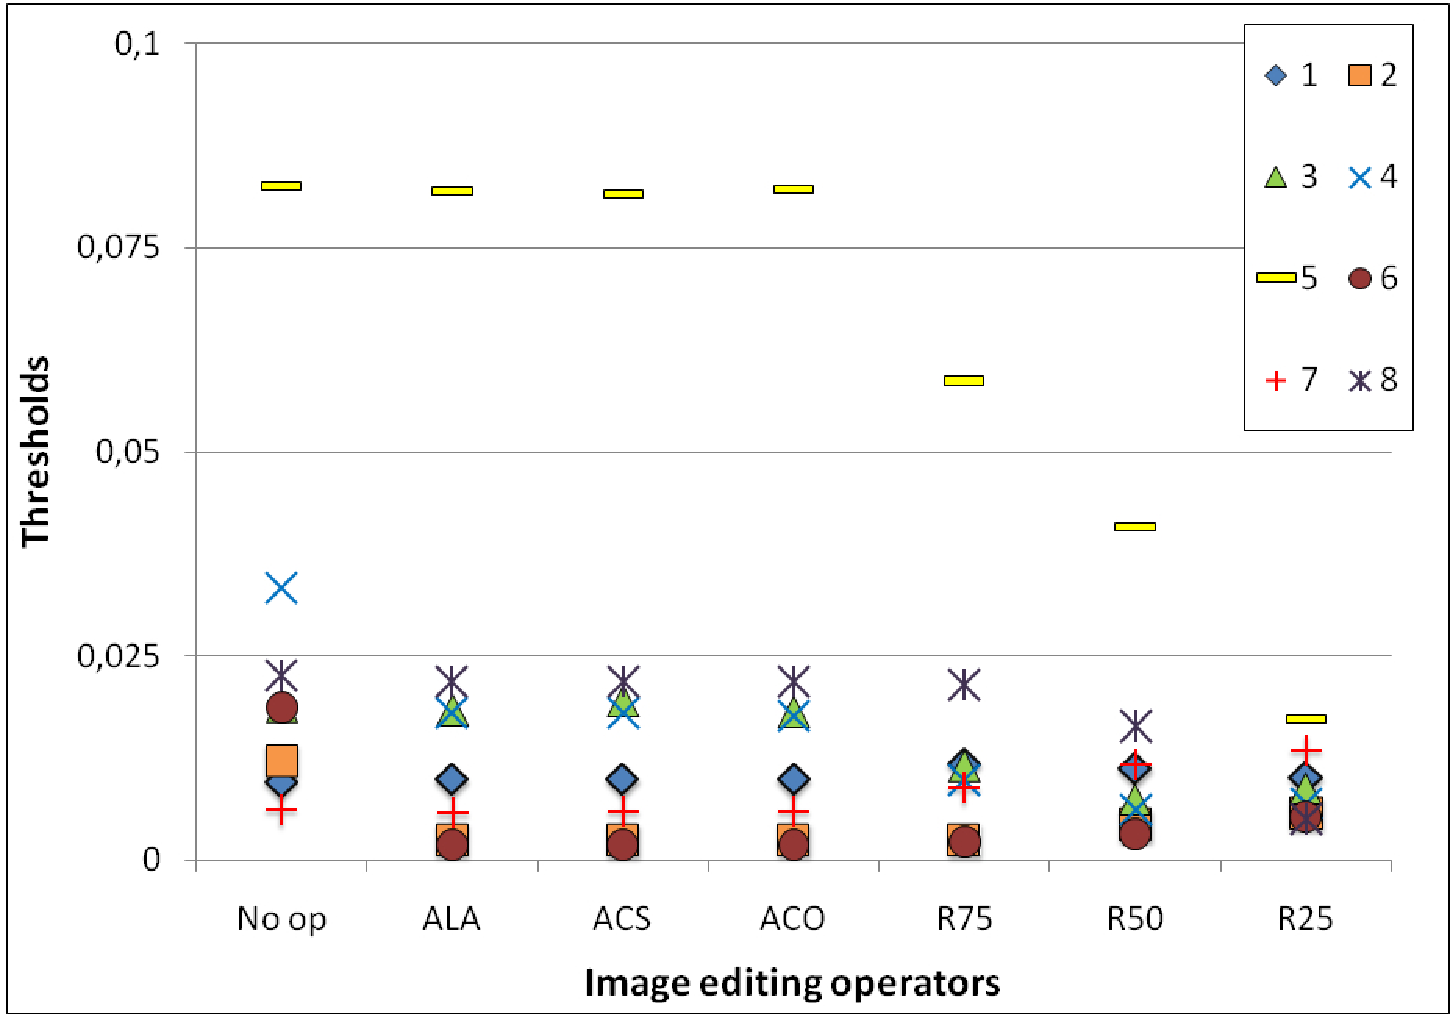
\includegraphics[width=12.0truecm]{ThresholdColor.pdf}}
% \centerline{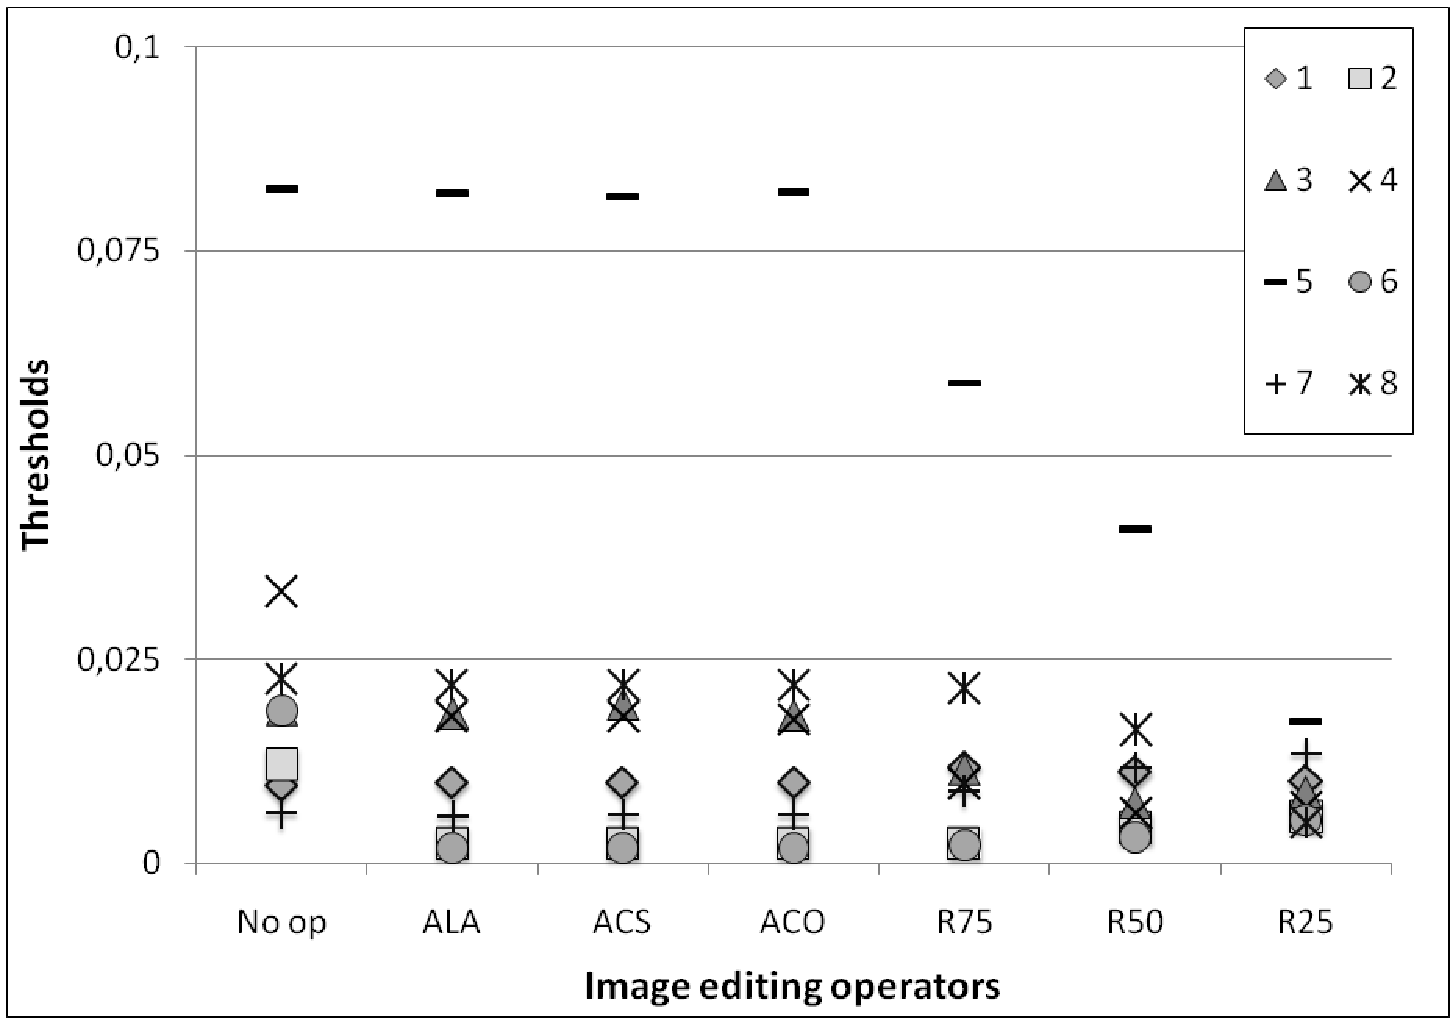
\includegraphics[width=10truecm]{ThresholdGray.pdf}}
 \caption{Thresholds values used according to the pre-processing operators being tested.}
 \label{thresholdsChart}
 \end{figure*}



\subsection{Experiment 3}\label{exp3}
In our previous experiment we have seen that if we try to classify pre-processed pictures using a classifier that has been tuned for unmodified pictures, the identification method by \Lukas\ may fail, in some cases, with a very high probability.  These failures are mostly due to the alteration of the pattern noise existing in a processed picture. This alteration implies a smaller correlation with the reference pattern noise. A natural solution to this problem consist in lowering the decision threshold used during the classification, so to correctly identify also pictures with smaller correlations. The results, documented in Table \ref{db8AutoEXP}, show a significant improvement on the quality of the classification, with respect to the second experiment. In this case, we have been able to obtain FRR rates which are very similar to those experienced with our first experiment. However, such a result comes at a cost. The new decision thresholds are, in some cases, much lower than the original ones. For example, we had to lower the decision threshold related to camera $5$ to more than the $90\%$ of its original value, thus raising the possibility of wrong classifications on larger data sets.

The same behavior can be noted when using the R75, R50, and R25 operators. As shown in Table \ref{resize75_50_25}, even for these operators, the thresholds change without any correlation with the percentage of resize. In other words, what we should have expected with this experiment is that reducing the image size will decrease the correlation index. In practice this not happens for all the cameras because we notice different behavior for some cameras. In particular, the threshold of the camera with ID 8 goes down while those for camera with ID 7 increase.

%
%% figura indicante la variazione della soglia 
% \begin{figure*}[htb]
% \centerline{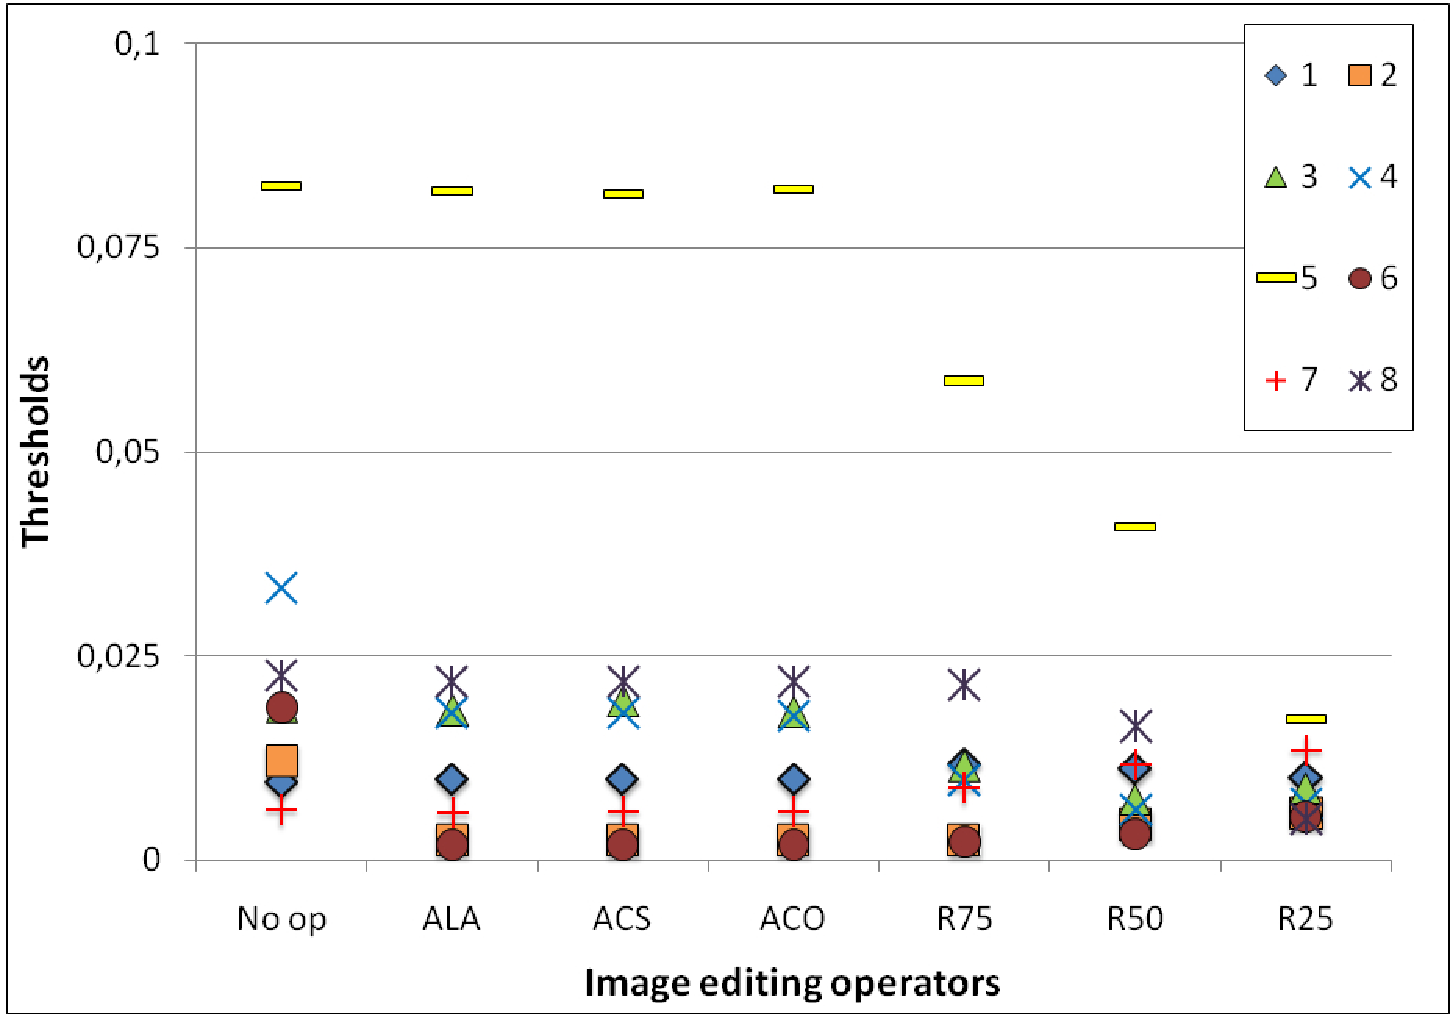
\includegraphics[width=10.5truecm]{ThresholdColor.pdf}}
%% \centerline{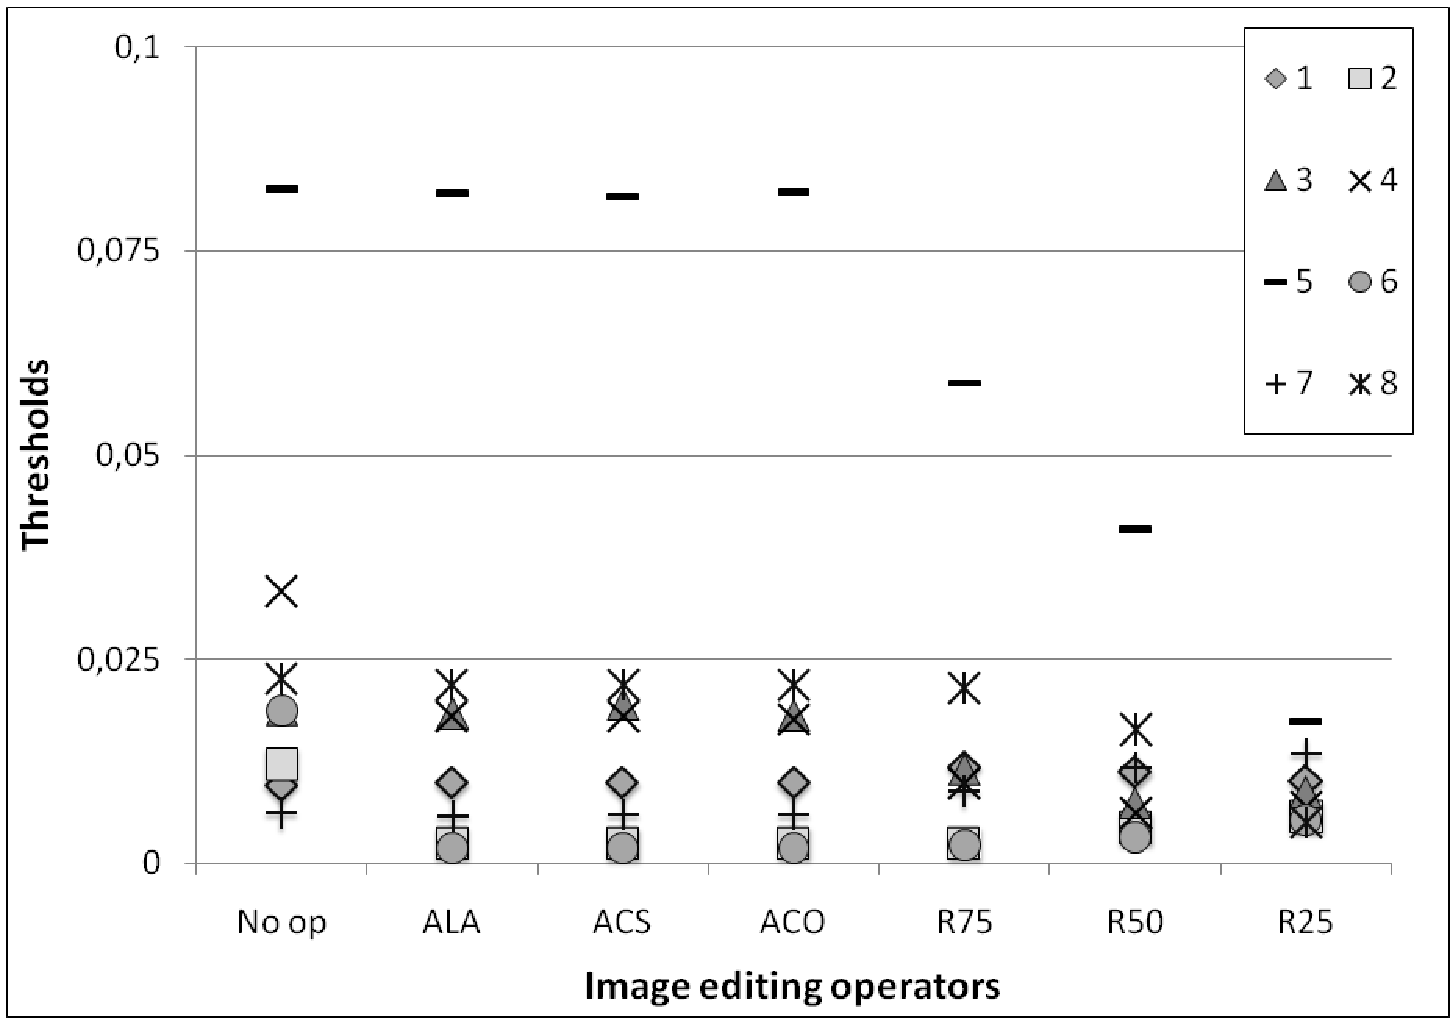
\includegraphics[width=10truecm]{ThresholdGray.pdf}}
% \caption{Thresholds values used according to the pre-processing operators being tested.}
% \label{thresholdsChart}
% \end{figure*}
%

%
%\begin{table*}[htb]
%\centering
%\caption{Decision thresholds, FRR and number of images rejected on the red channel for the experiments ALA, ACS and ACO.}
%\begin{tabular}{  | p{1.8cm}  | p{1.8cm}  | p{1.8cm}  |  p{1.8cm} | p{1.8cm}  | p{1.8cm} | p{1.8cm}  |} 
%\hline
%
%& \multicolumn{2}{|c|}{ \textbf{ALA} } & \multicolumn{2}{|c|}{ \textbf{ACS} }  & \multicolumn{2}{|c|}{ \textbf{ACO} }\\ \hline
%{\textbf{ID}}& Decision threshold & Images rejected (FRR) & Decision threshold& Images rejected (FRR) & Decision threshold& Images rejected (FRR)  \\ \hline
%
%1 &	0,0098	& 	|			& 0,0098			& |				&	0,0098		   	&		|	 \\
%2 &	0,0026 	& 	2 (0,0313)		& 0,0026			& 2 (0,0313)		&	0,0027		   	&		2 (0,0313)	 \\ 
%3 &	0,0184  	& 	4 (0,0625)		& 0,0195			& 4 (0,0625)		&	0,0182			&		4 (0,0625)  \\ 
%4 &	0,0180  	& 	1 (0,0156) 	&  0,0180			& 1 (0,0156)		&	0,0177			&		1 (0,0156) 	\\ 
%5 & 	0,0821  	&	|			& 0,0817			& |				& 	0,0822			& 		|  \\
%6 &	0,0018  	&	1 (0,0156) 	& 0,0018			& 1 (0,0156)		&	0,0019			&		1 (0,0156) \\ 
%7 &	0,0058  	&	|			& 0,0059			& |				&	0,0059			&		| \\
%8 &	0,0217  	&	|			& 0,0219			& |				&	0,0219			&		|	 \\ \hline \hline
%\multicolumn{2}{|c|}{total number of images rejected} & 8& & 8 & & 8 \\
%\hline
%\end{tabular}
%\label{db8AutoEXP}
%\end{table*}
%

%
%\begin{table*}[htb]
%\centering
%\caption{Decision thresholds, FRR and number of images rejected on the red channel for the experiments R75, R50 and R25.}
%\begin{tabular}{  | p{1.8cm}   | p{1.8cm} | p{1.8cm}  |  p{1.8cm} | p{1.8cm}  | p{1.8cm} | p{1.8cm}  |} 
%\hline
%& \multicolumn{2}{|c|}{ \textbf{R75} } & \multicolumn{2}{|c|}{ \textbf{R50} }  & \multicolumn{2}{|c|}{ \textbf{R25} }\\ \hline
%{\textbf{ID}}& Decision threshold& Images rejected (FRR) & Decision threshold& Images rejected (FRR) & Decision threshold& Images rejected (FRR)  \\ \hline
%
%1 &	0,0118	& 	|			& 0,0111			& |					&	0,0100		   	&		|	 \\
%2 &	0,0026 	& 	2 (0,0313)		& 0,0044			& 2 (0,0313)			&	0,0058		   	&		2 (0,0313)	 \\ 
%3 &	0,0115  	& 	4 (0,0625) 	& 0,0074			& 4 (0,0625)			&	0,0088			&		4 (0,0625)  \\ 
%4 &	0,0097  	& 	1 (0,0156) 	& 0,0061			& 1 (0,0156)			&	0,0070			&		1 (0,0156) 	\\ 
%5 &   0,0588  	&	|			& 0,0409			& |					& 	0,0173			& 		|  \\
%6 &	0,0022  	&	1 (0,0156)		& 0,0031			& 1 (0,0156)			&	0,0052			&		3 (0,0469) \\ 
%7 &	0,0088  	&	| 			& 0,0118			& |					&	0,0135			&		| \\
%8 &	0,0214  	&	|			& 0,0164			& |					&	0,0050			&		1 (0,0156)\\ \hline \hline
%\multicolumn{2}{|c|}{total number of images rejected} & 8 & & 8 & & 11 \\
%\hline
%\end{tabular}
%\label{resize75_50_25}
%\end{table*}

%Analyzing Figure~\ref{thresholdsChart} can be noted that most of the cameras made by Canon have lower decision thresholds and experience only a slight decrement in the performance of the classification, when compared to other cameras. 
%This is probably due to a better quality control of their sensors. This is further confirmed by fact that the cameras with the lower thresholds are the two reflex and are the only ones equipped with a CMOS sensor.

Analyzing Figure~\ref{thresholdsChart} can be noted that no relation exists between the thresholds and the market sector of the camera models used.
Moreover, each camera is independent from other cameras since it presents its own threshold. Indeed, the thresholds differ for the same camera model (cameras 3 and 4) and for camera models probably equipped with the same sensor (cameras 1 and 2). 
Furthermore, the figure points out how the results of the operators are strictly dependent on the camera, showing that the operators do not linearly affect all the cameras.
 


\section{Conclusions}
\label{sec:conc}

In this paper, we evaluated the effectiveness of the source camera identification technique from Luk{\' a\v s} {\em et  al.}, when using, as input, pictures that have altered by means of commonly-used image processing operators. The result of our experiments show, first of all, that the classification of the altered images may perform very bad if the classifier has been tuned using unmodified images (see subsection~\ref{exp2}). This problem can be fixed by tuning the classifier according to a data set of altered images and, consequently, by lowering the decision thresholds used to establish if a picture has been taken with a given camera.  In this new configuration, the Luk{\' a\v s} method confirms its effectiveness (see subsection~\ref{exp3}), even when processing altered images, although there are processing operators, like resizing and/or increasing the compression factor of a jpeg picture, which seems to have a bad effect on the results of the classification. 

% Umberto: questa parte qui non mi � molto chiara
%Moreover, this issue raises the problem about which decision threshold to use during a real investigation on a photographic exhibit. In fact, if the threshold computation would have been  performed on a set of images ``unaltered'', then the obtained threshold value could have been greater than the  correlation index of a given, altered, image under scrutiny. Otherwise, if the computation of the decision threshold would be computed on a set of images altered, then in such a case the FRR would be increased.
 

As a side effect of our experimentation, we experienced that the usage of an operator of type {\em Resize} seems to be preferable to an operator of type {\em Crop} when calculating the correlation between two images of different sizes. 


%
% in oder to calculate the correlation between an image
%and a Reference Pattern, uses the Crop operator. Our experiments~(see subsection~\ref{exp1}) 
%demonstrated that the use of the Resize operator instead of Crop gives a slight improvement to 
%the Luk{\' a\v s} {\em et  al.} technique.

%Il metodo utilizzato da Luk{\' a\v s} {\em et  al.} prevede l'utilizzo dell'operazione di CROP per il computo della
%correlazione tra un'immagine e un Reference Pattern di diverse risoluzioni. I nostri esperimenti 
%(see subsection~\ref{exp1}) hanno dimostrato che l'utilizzo dell'operazione di RESIZE al posto del CROP
%comporta un leggero miglioramento alla loro tecnica.
%

%The authors, starting from the Luk{\' a\v s} {\em et  al.} research have conducted a deep analysis of such method
%and have evaluated it when the images under examination have been altered (eventually willfully) by using simple
%operations of digital photo editing. The result of the second experiment~(see subsection~\ref{exp2}) shows that 
%the classification of the altered images does not work well if the thresholds have been computed on a unaltered data set.
%So the authors decided to further improve their experimental work by setting up another test-bed in which new thresholds
%are computed on altered data sets.
%The results of the third experiment~(see subsection~\ref{exp3}) confirmed 
%the effectiveness of the Luk{\' a\v s} method although have pointed out that the threshold decreases as shown
%in Figure~\ref{thresholdsChart}.

%Gli autori partendo dalla tecnica di Luk{\' a\v s} {\em et  al.} hanno effettuato un'attenta analisi di tale metodologia
%e l'hanno sottoposta all'esame nel caso in cui le immagini sotto osservazione siano state alterate (eventualmente
%in modo deliberato) mediante semplici operazioni di editing fotografico. I risultati del secondo esperimento 
%(see subsection~\ref{exp2}) hanno dimostrato l'efficacia del metodo di Luk{\' a\v s} {\em et  al.} bench� hanno 
%mostrato che la soglia di accettazione si abbassa come mostrato in figura \ref{thresholdsChart}.

The drop of the threshold involves, nonetheless, some problems while choosing which threshold to use 
during a real investigation on a photographic exhibit. In fact, if the threshold computation would have been  performed on a set of images ``unaltered'', then the obtained threshold value could have been greater than the  correlation index of a given, altered, image under scrutiny. Otherwise, if the computation of the decision threshold would be computed on a set of images altered, then in such a case the FRR would be increased.
 
%L'abbassamento della soglia comporta in ogni caso problemi per la scelta di quale soglia utilizzare nella fase
%investigativa. Infatti, se il computo delle soglie viene effettuato su di un campione di immagini non ``alterato'',
%allora il valore della soglia ottenuto potrebbe essere maggiore dell'indice di correlazione di una data immagine
%sotto investigazione che abbia subito delle alterazioni.
%D'altro canto per�, se per il computo della soglia di decisione venisse presa quella calcolata su di un campione
%di immagini ``alterato'', in tale caso aumenterebbe il tasso di falso rifiuto (FRR).

We intend to proceed with our research by increasing the number of cameras and pictures involved in our experiments, by implementing some other classification techniques and, finally, by extending our experimentations to pictures that have been previously published and processed, and then downloaded, from social networks and photo publishing sites such as Facebook and PicasaWeb.

% use section* for acknowledgment
\section*{Acknowledgment}
The authors would like to thank the chief of the CNCPO, V.Q.A.~Dr.~Elvira D'Amato, along with her group, for their valuable 
suggestions during the research
%The authors would like to thank the members of the CNCPO for their valuable suggestions during the research
phases. Their needs, questions and doubts coming from real and day-by-day investigations have encouraged the
authors to further improve this work. An earthy thanks goes to the group of graduate students
that with their effort helped us to carry out the research.

\bibliographystyle{IEEEtran}
\balance
\bibliography{if}


% that's all folks
\end{document}


